\documentclass[a4paper,11pt]{article}
\usepackage[T1]{fontenc}
\usepackage[utf8]{inputenc}
\usepackage[ngerman]{babel}
\usepackage{amsmath,amssymb}
\usepackage[margin=2.2cm]{geometry}
\usepackage{graphicx}
\usepackage{tikz}
\usepackage[most]{tcolorbox}
\usepackage[hidelinks]{hyperref}
\setlength{\parindent}{0pt}
\setlength{\parskip}{5pt}
\providecommand{\explainmode}{0}
\newif\ifexplain
\ifnum\explainmode=1 \explaintrue\fi
\newcommand{\aufgabe}[1]{\section*{Aufgabe #1}}
\newcommand{\angabe}[1]{\textit{#1}\par\smallskip}
\newcommand{\why}[1]{\text{#1}}
\newtcolorbox{erklbox}{colback=blue!4,colframe=blue!40,breakable,boxrule=.5pt,title=Erklärung}
\newcommand{\explain}[1]{\ifexplain\begin{erklbox}#1\end{erklbox}\fi}
\newcommand{\explainfig}[1]{\ifexplain\begin{center}#1\end{center}\fi}
\begin{document}
\begin{center}
{\Large Übungsblatt 03: POP3 und HTTP mit Python Sockets}\\
PR Rechnernetze und Netzwerkprogrammierung 621.801/621.802\\
Raphael Bleier, Gruppe YY, WS 2026/2027
\end{center}

\aufgabe{3.1}
\angabe{POP3 anhand RFC 1939 untersuchen: Arbeitsablauf, Sicherheit und Unterschied zwischen single-line und multi-line response. Mit IMAP vergleichen.}

Nach dem TCP-Verbindungsaufbau schickt der Server eine Begrüßung mit \texttt{+OK}. Es folgen drei Zustände:
\begin{enumerate}
\item AUTHORIZATION: \texttt{USER} und \texttt{PASS} übermitteln die Anmeldung. Der Server prüft die Daten und sperrt den Maildrop exklusiv. Erst bei Erfolg beginnt TRANSACTION (RFC 1939, Abschnitt 4).
\item TRANSACTION: \texttt{STAT} nennt Anzahl und Gesamtgröße; \texttt{LIST} listet Größen und \texttt{RETR n} liefert Nachricht $n$. \texttt{DELE n} markiert eine Nachricht zunächst nur. \texttt{RSET} entfernt diese Markierungen (Abschnitt 5).
\item UPDATE: \texttt{QUIT} aus TRANSACTION übernimmt die Löschungen und beendet die Verbindung. Bei einem Abbruch ohne dieses \texttt{QUIT} darf der Server die Markierungen nicht übernehmen (Abschnitt 6). \texttt{QUIT} vor der Anmeldung beendet die Verbindung ohne UPDATE.
\end{enumerate}
\explain{Der Maildrop ist hier der Vorrat an Nachrichten eines Benutzers. Die Sperre verhindert, dass zwei Sitzungen gleichzeitig verschiedene Löschstände auf denselben Vorrat anwenden. Abrufen heißt noch nicht Löschen: Das sind getrennte Kommandos.}

\explainfig{\begin{tikzpicture}[every node/.style={draw,rounded corners,align=center,font=\small},>=stealth]
\node (a) at (0,0) {AUTHORIZATION};
\node (t) at (5,0) {TRANSACTION};
\node (u) at (10,0) {UPDATE};
\draw[->] (a)--node[above,draw=none]{Login und Lock}(t);
\draw[->] (t)--node[above,draw=none]{QUIT}(u);
\end{tikzpicture}}

Unverschlüsseltes POP3 (üblicherweise auf Port 110) schützt weder Passwort noch Nachrichten. Ein Mitschnitt kann beides offenlegen. Für echte Zugänge ist TLS mit Zertifikatsprüfung nötig, etwa implizites TLS auf Port 995. APOP aus RFC 1939 ist keine Verschlüsselung der Maildaten und kein Ersatz für TLS. Der hier implementierte Server ist auf einen lokalen Labortest ohne TLS beschränkt.
\explain{Authentifizierung und Verschlüsselung lösen verschiedene Probleme. Ein richtig geprüftes Passwort verhindert nicht, dass jemand den unverschlüsselten Transport mitliest. Deshalb werden im Versuch ausschließlich die vorgegebenen Testdaten verwendet.}

Eine single-line response enthält genau eine Statuszeile mit \texttt{+OK} oder \texttt{-ERR}. Eine erfolgreiche multi-line response beginnt ebenfalls mit einer Statuszeile, enthält anschließend Datenzeilen und endet mit einer Zeile, die nur einen Punkt enthält. Jede Zeile endet mit CRLF. Datenzeilen mit führendem Punkt erhalten einen zusätzlichen Punkt; der Client entfernt beim Lesen genau diesen einen Punkt. \texttt{LIST} ist ohne Argument mehrzeilig, \texttt{LIST 1} einzeilig. Eine negative Antwort hat keinen anschließenden Datenblock.
\explain{Die Punktzeile ist ein Endezeichen, keine Nachrichtendatei. Eine echte Mailzeile mit einem einzelnen Punkt wird daher als zwei Punkte übertragen. Auch Leerzeilen am Nachrichtenende gehören zum Inhalt und dürfen nicht durch pauschales Abschneiden verloren gehen.}

IMAP verwendet getaggte Kommandos und Abschlüsse sowie ungetaggte Antworten. Literale können eine explizite Bytelänge haben; sie werden nicht durch POP3-Dot-Stuffing eingerahmt. IMAP unterstützt serverseitige Ordner, Flags und Synchronisierung mehrerer Geräte. POP3 konzentriert sich auf den Abruf. Serverkopien können dabei erhalten bleiben, wenn der Client keine Löschung verlangt. Grundlage: RFC 9051 sowie LV-Folien 36--37.
\explain{Ein Tag wie \texttt{A001} ordnet bei IMAP das Ergebnis einer Anfrage zu. Das ist etwas anderes als die Nachrichtennummer bei POP3. Für den Vergleich zählt vor allem, wo Ordner und Lesestatus verwaltet werden.}

\aufgabe{3.2}
\angabe{Einen POP3-Client mit Standardbibliothek und Socket-Kommunikation schreiben. Anmelden, alle Nachrichten auflisten, eine Nachricht abrufen und die Verbindung ordentlich abbauen. Mit einem geeigneten Server testen; lokale Server oder ein TLS-Tunnel sind erlaubt.}

Abgabe: \texttt{pop3\_client.py}. Der Ablauf lautet Begrüßung, \texttt{USER}, \texttt{PASS}, \texttt{LIST}, \texttt{RETR n}, \texttt{QUIT}. Statusfehler werden abgefangen, CRLF und Dot-Stuffing ausgewertet. Das Passwort wird verdeckt abgefragt. Der Client schließt Reader und Socket auch nach einer fehlerhaften Begrüßung oder einem fehlgeschlagenen \texttt{QUIT}.
\explain{TCP liefert einen Bytestrom, keine vollständigen Antworten pro Empfangsaufruf. Der gepufferte Reader setzt deshalb auch fragmentierte Zeilen wieder zusammen. Die Statusprüfung kommt vor dem Lesen eines Datenblocks, weil eine Fehlermeldung gerade keinen mehrzeiligen Block ankündigt.}

Der Test gegen den lokalen Server mit der Original-Datenbank bestätigte vier Nachrichten. \texttt{LIST} meldete 184, 185, 154 und 164 Bytes. Der erste \texttt{RETR}-Abruf stimmte bytegenau mit der CRLF-normalisierten Originalnachricht überein. Weitere Tests prüfen fragmentierte Antworten, Punktzeilen, EOF und die Abwehr von Zeilenumbrüchen in Kommandos.
Eine Gegenprobe mit dem im Blatt verlinkten GoPop3Server bestätigte Anmeldung, \texttt{LIST}, \texttt{RETR} und \texttt{QUIT}. Dieser separate Referenzserver lieferte zwei Nachrichten mit 151 und 115 Bytes; der erste Betreff war \glqq Hello Alice\grqq. Der Versuch lief in einem isolierten lokalen Netzwerk.
\explain{Die Größen beziehen sich auf die Nachricht mit CRLF, nicht auf Statuszeilen, zusätzliche Punkte oder die abschließende Punktzeile. Der Vergleich mit den Originalbytes prüft daher eine andere Eigenschaft als ein bloßer Vergleich des sichtbaren Mailtexts.}

\aufgabe{3.3}
\angabe{Einen minimalen POP3-Server mit der bereitgestellten Klasse SampleDataBase.py implementieren. Die Nachrichten sollen im Posteingang eines echten Mailprogramms erscheinen. Pro Benutzer einen Thread verwenden; parallele Benutzer zulassen. Client und Server praktisch testen und den Ablauf mit Screenshots dokumentieren. RFC 1939 und RFC 2449 beachten.}

Abgabe: \texttt{pop3\_server.py}. Die externe Datenbank wird über \texttt{authenticate} und \texttt{get\_messages} benutzt. Pro Verbindung läuft ein Thread. Ein Lock pro Benutzer verhindert zwei gleichzeitige Transaktionen auf demselben Maildrop. Unterschiedliche Benutzer bleiben parallel bedienbar.
\explain{Die Threads gehören zu Verbindungen, nicht dauerhaft zu Konten. Wenn sich derselbe Benutzer später erneut verbindet, übernimmt ein neuer Sitzungsthread die Bearbeitung, während der gemeinsame Benutzer-Lock weiterhin verhindert, dass zwei gleichzeitig angemeldete Sitzungen widersprüchliche Löschungen am selben Maildrop vornehmen. Das Annehmen weiterer Verbindungen bleibt davon getrennt.}

Implementiert sind \texttt{USER}, \texttt{PASS}, \texttt{STAT}, \texttt{LIST}, \texttt{RETR}, \texttt{DELE}, \texttt{RSET}, \texttt{NOOP} und \texttt{QUIT}; zusätzlich \texttt{CAPA}, \texttt{TOP} und \texttt{UIDL}. Nachrichtennummern bleiben innerhalb einer Sitzung stabil. \texttt{UIDL} nutzt einen Hash aus Original-ID und Inhalt. Löschungen werden nur bei \texttt{QUIT} übernommen. Die Datenbankdatei bleibt unverändert; ohne dauerhafte Löschschnittstelle besteht der Löschstand nur im laufenden Serverprozess. Das Inaktivitätstimeout beträgt 600 Sekunden.
\explain{\texttt{DELE} entfernt zunächst keine Datei. Die Sitzung merkt sich nur die Nummer. Erst beim Wechsel nach UPDATE wird die ursprüngliche Datenbank-ID in den lokalen Löschstand geschrieben. Dadurch kann ein abgebrochener Download keine bereits markierten Nachrichten versehentlich entfernen.}

GUI-Test: Claws Mail 4.3.1 mit einem frischen Profil, POP3 auf Loopback, Port 11110, Testbenutzer aus der Original-Datenbank und ohne TLS. Die Option zum Löschen nach Abruf war ausgeschaltet. Nach dem Abruf erschienen vier Nachrichten im Posteingang. Die erste Nachricht wurde geöffnet. Der Screenshot zeigt die Betreffe sowie Header und Text dieser Nachricht. Die Standardbibliothek \texttt{poplib} wurde zusätzlich als unabhängiger Protokollclient verwendet.

% grafik-verlangt
\begin{center}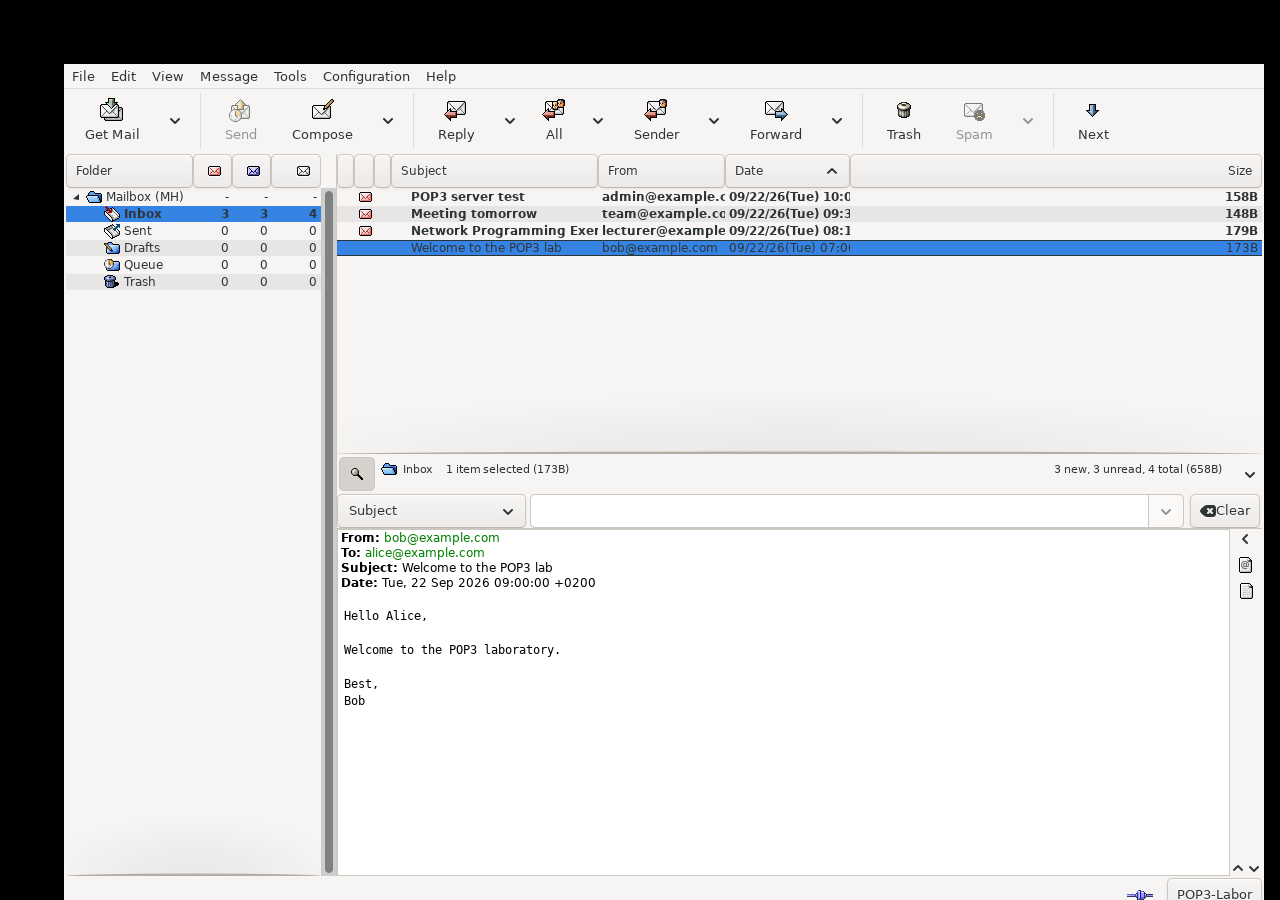
\includegraphics[width=\linewidth]{screenshots/pop3-claws.png}\end{center}

\aufgabe{3.4}
\angabe{Einen Single-Thread-HTTP/0.9-Server schreiben. Port (Vorgabe 80) und document root als Kommandozeilenparameter anbieten. Einzelne Dateien liefern, für Verzeichnisse index.html verwenden und bei Fehlern ohne Rückmeldung schließen. Mit documentRoot.zip und unterschiedlichen Browsern testen. Werden die Daten richtig angezeigt?}

Abgabe: \texttt{http\_server.py --mode 09}. Dieser Modus behandelt Verbindungen nacheinander. Akzeptiert wird \texttt{GET /pfad} mit CRLF. Die Antwort besteht nur aus den Dateibytes; danach wird die Verbindung geschlossen. Pfade werden dekodiert, aufgelöst und auf das Basisverzeichnis beschränkt. Fehlende Dateien und ungültige Anfragen liefern keine Antwortbytes.
\explain{HTTP/0.9 kennt in dieser einfachen Form weder Statuszeile noch Header. Der Client erkennt das Ende deshalb am Verbindungsabbau. Ein HTTP/1.0-Statuscode als Fehlermeldung würde gerade nicht zum geforderten Verhalten passen.}

Socket-Tests bestätigen \texttt{index.html}, Unterverzeichnisse und binäre Dateiinhalte. Kodierte Traversal-Versuche und Symlinks außerhalb des document root werden abgewiesen. Der document root muss während des Betriebs unter eigener Kontrolle bleiben; der Server bietet keine Betriebssystem-Sandbox gegen gleichzeitige fremde Dateisystemänderungen.
\explain{Ein Präfixvergleich von Pfadzeichenketten reicht nicht. Weil auch ein scheinbar harmloser Link auf einen fremden Ordner aus dem Basisverzeichnis herausführen kann, wird zuerst das tatsächliche Ziel aufgelöst und danach geprüft, ob dieses Ziel noch innerhalb des erlaubten Verzeichnisses liegt. Erst danach darf die Datei geöffnet werden.}

Mit Chromium 156.0.8078.4 und Firefox 157.0 wird die Seite in diesem Modus nicht richtig angezeigt. Die Browser senden aktuelle Request-Zeilen, die der strikte Zweitoken-Parser ablehnt. Chromium meldete \texttt{ERR\_EMPTY\_RESPONSE}; Firefox lieferte im Navigationsaufruf \texttt{NS\_ERROR\_NET\_RESET}. Der Firefox-Screenshot zeigt die leere Antwort als Browserfehler. Dieses Testergebnis wurde nicht als erfolgreiche Darstellung gewertet.

\explainfig{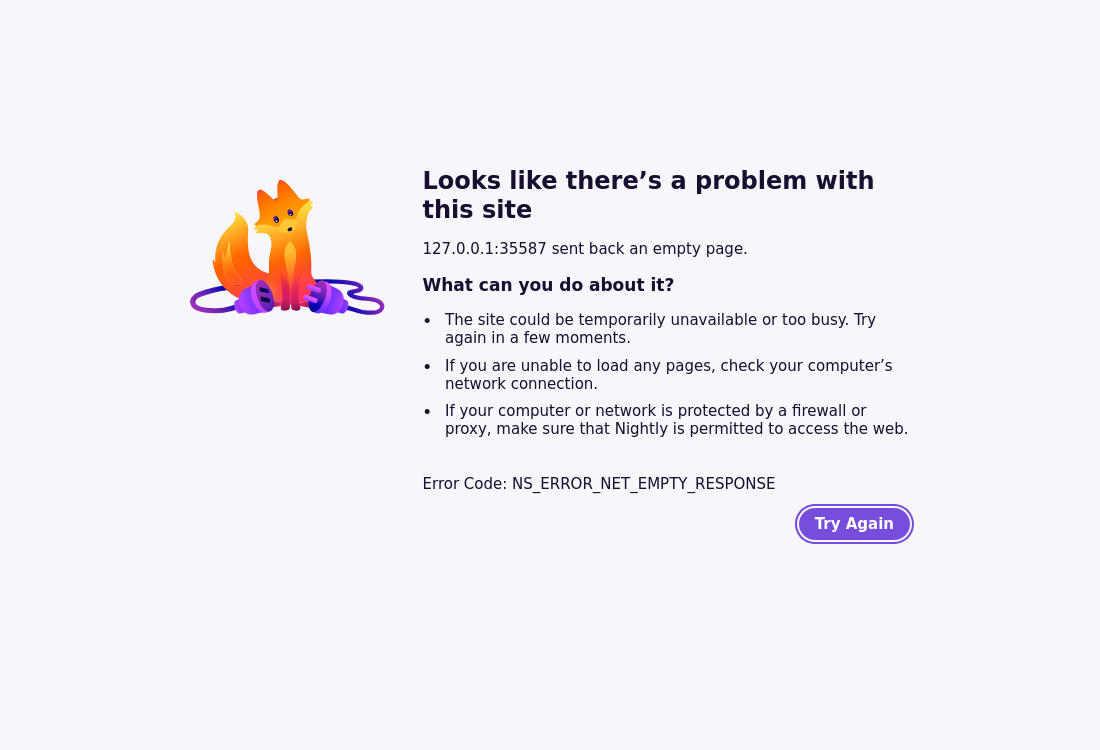
\includegraphics[width=.85\linewidth]{screenshots/http09-firefox.png}}

\aufgabe{3.5}
\angabe{Den Server erweitern: jede Anfrage durch einen neuen Thread behandeln, HTTP/1.0 und persistente Verbindungen unterstützen. Zeitpunkt, Request-Typ, Client-IP und Clientport zentral in einem eigenen Thread alle fünf Sekunden ausgeben. Geeignet synchronisieren.}

Abgabe: \texttt{http\_server.py --mode 10}. Ein Verbindungsthread liest vollständige Anfragen. Für jede Anfrage startet er einen eigenen Worker. Vor dem nächsten Request auf derselben Verbindung wartet er auf dessen Antwort. Andere Verbindungen arbeiten parallel. \texttt{GET} liefert Dateidaten, \texttt{HEAD} nur die passenden Header.
\explain{Ein Thread pro Verbindung allein wäre hier nicht die wörtliche Anforderung. Deshalb gibt es zusätzlich den Request-Worker. Die Reihenfolge bleibt trotzdem fest: Antwort zwei darf auf derselben TCP-Verbindung nicht mitten in Antwort eins geschrieben werden.}

Antworten verwenden \texttt{HTTP/1.0}, \texttt{Content-Length}, \texttt{Content-Type} und \texttt{Connection}. Nur explizites Keep-Alive hält die Verbindung offen; \texttt{close} hat Vorrang. Die Grenze liegt bei 100 Requests beziehungsweise fünf Sekunden Inaktivität. HTTP/1.1-Request-Zeilen werden für moderne Clients akzeptiert, aber mit HTTP/1.0 beantwortet. Request-Bodies, Chunked-Encoding und doppelte Header werden abgelehnt. Fehler erhalten 400, 403, 404 oder 405 entsprechend der Ursache.
\explain{Eine persistente Verbindung endet nicht nach jeder Datei. Der Client braucht deshalb die exakte \texttt{Content-Length}, um das Ende der Dateibytes und damit den möglichen Beginn der nächsten Antwort zu finden, ohne dafür auf einen Verbindungsabbruch warten zu müssen. Request-Bodies werden nicht still ignoriert: Übrig gebliebene Bodybytes könnten sonst als nächste Anfrage gelesen werden.}

Die Handler schreiben ausschließlich Logereignisse in eine threadsichere Queue. Ein separater Logger-Thread sammelt sie und schreibt alle fünf Sekunden Zeitstempel, Methode, Clientadresse und Clientport. Beim regulären Beenden wird der Rest ausgegeben. Nur dieser Thread schreibt den Logstrom. Passwörter und Header werden nicht erfasst.
\explain{Die Queue trennt das Bearbeiten der Anfrage von der Ausgabe. Statt dass jeder Request-Thread auf ein langsames Terminal und einen gemeinsam gehaltenen Datei-Lock warten muss, legt er seinen Eintrag in der Queue ab und überlässt das spätere Sammeln und Schreiben vollständig dem Logger. Dessen Puffer verändert kein anderer Thread.}

Im HTTP/1.0-Modus lieferten Chromium und Firefox den Text \glqq It works...!\grqq\ und beide Bilder korrekt. Die Bildprüfung bestätigte geladene Bilder mit positiver natürlicher Breite. Zwei Requests auf derselben TCP-Verbindung und 16 parallele Requests wurden separat getestet. Die Browser-Aufnahmen liegen im Ordner \texttt{screenshots}; das Erklär-PDF enthält zusätzlich die Chromium-Darstellung.

\explainfig{
\includegraphics[width=.85\linewidth]{screenshots/http10-chromium.png}}

\section*{Prüfung, Quellen und Abgabe}
21 Tests liefen mit Python 3.14.7 erfolgreich durch; Browsersteuerung mit Python 3.11.15. Getestet wurden Anmeldung, Dot-Stuffing, Größen, Sperren, Lösch-Commit, Rollback, Framing, Pfadgrenzen, HTTP-Fehler, Keep-Alive, Parallelität und Logging. Startbefehle und Einzelheiten stehen in \texttt{README.md}. Die Programme und Tests sind Teil der Abgabe.

Grundlagen: Moodle-Blatt 03; bereitgestellte Datenbankschnittstelle und document root; LV-Unterlage \texttt{rn-chapter-2}, Folien 10--11 und 36--37. Normative Quellen: \href{https://www.rfc-editor.org/rfc/rfc1939}{RFC 1939}, Abschnitte 3--7; \href{https://www.rfc-editor.org/rfc/rfc2449}{RFC 2449}, Abschnitte 4--6; \href{https://www.rfc-editor.org/rfc/rfc1945}{RFC 1945}, Abschnitte 5--6; \href{https://www.rfc-editor.org/rfc/rfc8314}{RFC 8314} zur TLS-Einordnung und \href{https://www.rfc-editor.org/rfc/rfc9051}{RFC 9051} zu IMAP.

Moodle nennt für beide Gruppen den 17.11.2026, 08:00 Uhr (Stand 19.10.2026). Die Gruppennummer ist noch nicht bekannt und bleibt als YY markiert. Es wurde nichts auf Moodle eingereicht.

KI-Kennzeichnung laut Aufnahmefolien: Hermes Agent v0.21.5, Modell \texttt{gpt-6.1-sol}, verwendet am 19.10.2026 für Code, Texte und Tests. Die Python-Dateien nennen die jeweiligen Arbeitsaufträge. Alle genannten Testresultate und Screenshots stammen aus tatsächlich ausgeführten Programmen.
\end{document}
